\justy{Poniżej zaprezentowano uproszczony diagram przepływu. Diagram podzielono na 3 obiekty: użytkownika aplikacji, klienta, czyli aplikację mobilną będącą pośrednikiem pomiędzy użytkownikiem, a serwerem, i serwer który obsługuje wszystkie zapytania i odpowiednio je przetwarza, zarządza sesjami i połączeniami.}

\begin{figure}[H]
	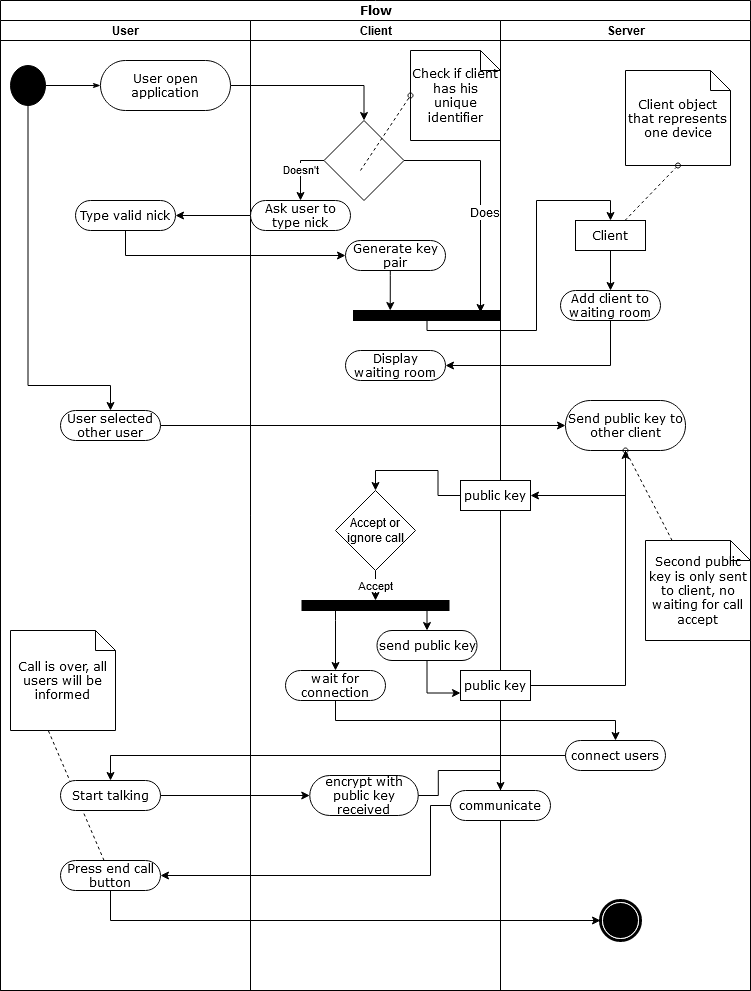
\includegraphics[width=\textwidth]{images/flow.png}
	\centering	
	\caption{\centering Uproszczony diagram przepływu przedstawiajacy inicjalizację sesji, a także dodania użytkownika do poczekalni.}
\end{figure}